\documentclass{beamer}

\mode<presentation>
{
	\usepackage{StyleFiles/Rome}
	\setbeamercovered{transparent}
}

\mode<handout>
{
	\usepackage{pgfpages}
	\pgfpagesuselayout{2 on 1}[a4paper,border shrink=5mm]
	\nofiles
}

\usepackage[english]{babel}

\setbeamertemplate{itemize subitem}{\tiny\raise1.5pt\hbox{\donotcoloroutermaths$ \blacktriangleright $}}

\title[PTracking open source library]{\Large PTracking: a distributed open source library that exploits a clustering technique to track multiple objects}

\subtitle{}

\author[Fabio Previtali]{\Large\textbf{Fabio Previtali}}

\date[May 13, 2013]{Oberseminar 2013\\Groningen, The Netherlands}

\begin{document}

\begin{frame}[plain]
	\titlepage
\end{frame}

\section{Outline}

\begin{frame}
	\frametitle{Outline}
	
	\begin{enumerate}
		\item Problem statement
		\item Multi-Clustered Particle Filtering
		\item Experimental evaluation
		\item BeeSafe project
		\item Research plan and future directions
	\end{enumerate}
\end{frame}

\section{Introduction}

\begin{frame}
	\frametitle{Challenging Problem}
	
	\begin{center}
		\begin{tikzpicture}
			\node at (0,0) [draw=white,ultra thick,inner sep=0pt]
			{
				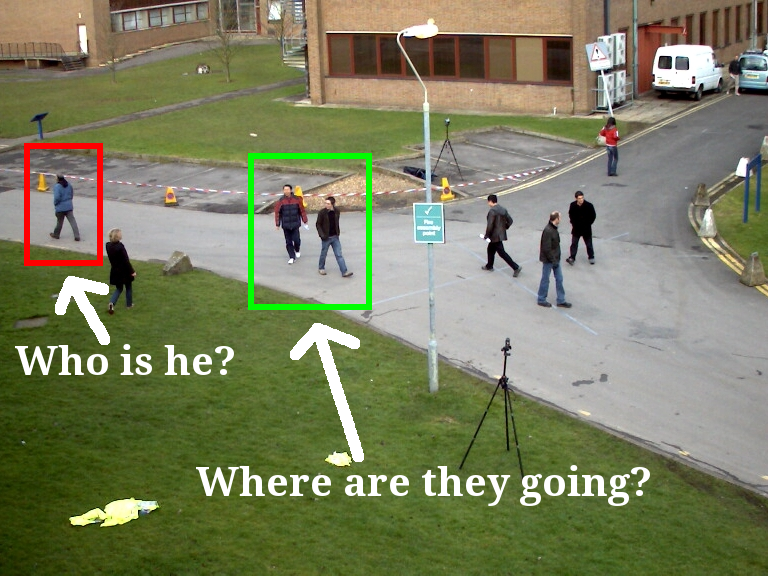
\includegraphics[width=\linewidth]{Figures/Problem.png}
			};
		\end{tikzpicture}
	\end{center}
\end{frame}

\begin{frame}
	\frametitle{Motivation}
	
	\vspace{0.2cm}
	
	\Large
	
	\begin{block}{Objective}
		\textbf{Understanding} the concept of human preference \textbf{allows} to perform higher levels
		of reasoning about future human actions. Likewise, the \textbf{knowledge} of a goal also gives
		information about \textbf{what} a person might do
	\end{block}
	
	\vspace{0.3cm}
	
	Example of application fields:
	\begin{itemize}
		\item Automatic video surveillance
		\item Human-Robot Interaction
		\item Domestic robots
	\end{itemize}
\end{frame}

\begin{frame}
	\frametitle{Contributions}
	
	\Large
	
	The main contributions of this thesis are:
	
	\begin{enumerate}
		\item \textbf{Distributed real-time} multiple object tracking
		\item \textbf{Asynchronous} and \textbf{fully} scalable design
		\item \textbf{Prediction} without prior scene semantics knowledge
		\item \textbf{Incremental} updates of the \emph{IRL} model over time
		\item \textbf{Non-uniform grids} for representing world state
		\item \textbf{Efficient} and \textbf{scalable} solution for on-robot implementation
	\end{enumerate}
\end{frame}

\begin{frame}
	\frametitle{Proposed Solution}
	
	\vspace{0.5cm}
	
	\begin{tikzpicture}
		\node at (0,0) [draw=white,ultra thick,inner sep=0pt]
		{
			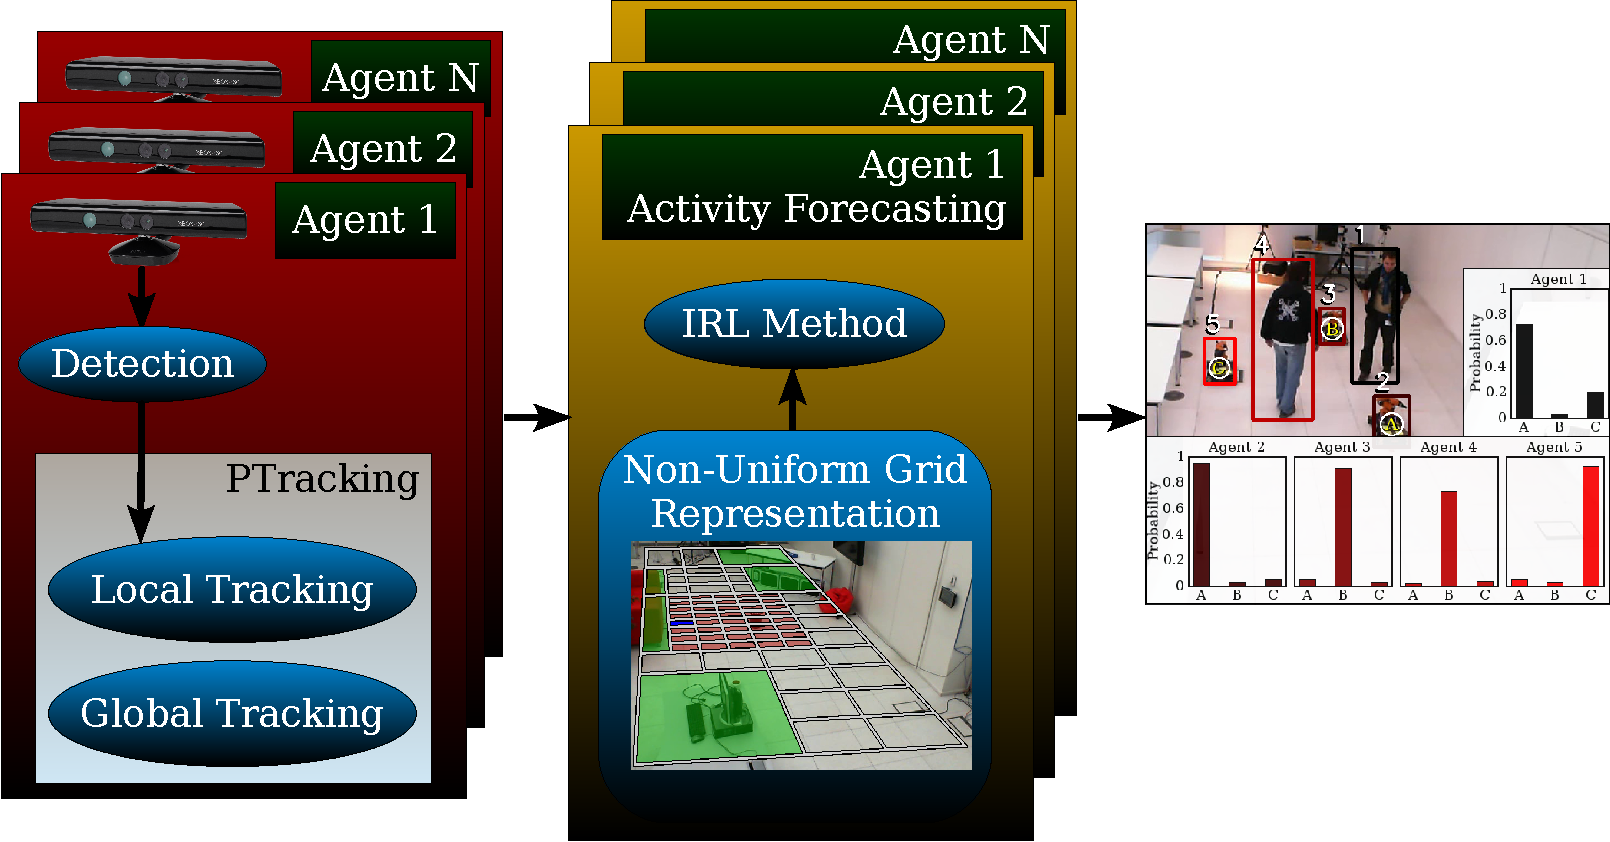
\includegraphics[width=\linewidth]{Figures/Architecture}
		};
	\end{tikzpicture}
\end{frame}

\section{Related Work}

\begin{frame}
	\frametitle{Related Work}
	\framesubtitle{Multi-object tracking}
	
	\Large
	
	\vspace{0.4cm}
	
	Multi-object tracking algorithms can be classified into two groups (Andriyenko \emph{et al.}):
	
	\vspace{0.2cm}
	
	\begin{itemize}
		\item \textbf{Global} (or \emph{offline}): formulating the tracking problem as an
			  optimization one, where all the trajectories within a temporal window are
			  optimized jointly
		\item \textbf{Recursive} (or \emph{online}): estimating the current state relying
			  only on the current observations and on the previous state
	\end{itemize}
\end{frame}

%\begin{frame}
%	\frametitle{Multi-Object Tracking}
%	\framesubtitle{Global methods}
%	
%	\Large
%	
%	\vspace{0.2cm}
%	
%	\begin{itemize}
%		\item \textbf{Berclaz} \emph{et al.} \cite{Berclaz11}: mathematically sound
%			  multiple object tracking framework based on a k-shortest path optimization
%			  algorithm
%		\vspace{0.1cm}
%		\item \textbf{Leal-Taix{\'e}} \emph{et al.} \cite{Leal11}: formulate a new graph
%			  model for the multiple object tracking challenge by minimizing a network flow
%			  problem
%		\vspace{0.1cm}
%		\item \textbf{Sharma} \emph{et al.} \cite{Sharma09}: adapting a Cluster-Boosted
%			  Tree based pedestrian detector to deal with the people tracking problem
%		\vspace{0.1cm}
%		\item ...
%	\end{itemize}
%\end{frame}
%
%\begin{frame}
%	\frametitle{Multi-Object Tracking}
%	\framesubtitle{Recursive methods}
%	
%	\Large
%	
%	\vspace{0.2cm}
%	
%	\begin{itemize}
%		\item \textbf{Breitenstein} \emph{et al.} \cite{Breitenstein11}: online method for
%			  multi-person tracking-by-detection in a particle filtering framework
%		\vspace{0.1cm}
%		\item \textbf{Yang} \emph{et al.} \cite{Yang09}: probabilistic appearance model
%			  method for tracking multiple people
%		\vspace{0.1cm}
%		\item ...
%	\end{itemize}
%\end{frame}

\begin{frame}
	\frametitle{Global vs Recursive Methods}
	
	\begin{table}[!t]
		\centering
		\begin{tabular}{ c | c | c | }
			\cline{2-3}
			& \textbf{Global Methods} & \textbf{Recursive Methods} \\ \hline
			
			\multicolumn{1}{|c|}{\textbf{Accuracy}} & medium/high & medium/high \\ \hline
			\multicolumn{1}{|c|}{\textbf{Precision}} & \textbf{high} & medium/high \\ \hline
			\multicolumn{1}{|c|}{\textbf{Robustness}} & \textbf{high} & medium/high \\ \hline
			\multicolumn{1}{|c|}{\textbf{Computational Load}} & high & \textbf{low}/medium \\ \hline
			\multicolumn{1}{|c|}{\textbf{Real-time}} & no & \textbf{yes}/no \\ \hline
		\end{tabular}
	\end{table}
	
	\vspace{0.4cm}
	
	Global methods are more precise and more robust but, on the other hand, they
	cannot run in a real system because:
	
	\begin{itemize}
		\item no information from the future are available (offline computation)
		\item frame rate not suitable for real-time applications
	\end{itemize}
\end{frame}

\section{PTracking Algorithm}

\begin{frame}
	\frametitle{PTracking algorithm}
	
	\vspace{0.6cm}
	
	\textbf{Global recursive update}
	
	\vspace{-0.4cm}
	
	\begin{eqnarray*}
	p(x_t|z_{1:t-1}^\mathcal{A}) &=& \int p(x_t|x_{t-1}) p(x_{t-1}|z_{1:t-1}^\mathcal{A})dx_{t-1}, \\
	p(x_t|z_{1:t}^\mathcal{A}) &=& \frac{p(z_t^\mathcal{A}|x_t) p(x_t|z_{1:t-1}^\mathcal{A})}{\int p(z_t^\mathcal{A}|x_t)p(x_t|z_{1:t-1}^\mathcal{A})dx_t}.
	\end{eqnarray*}
	
	\textbf{GMM parameters}
	
	\vspace{-0.1cm}
	
	\begin{equation*}
		\mu_t^c = \frac{\sum_{i=1}^N x_t^{(i)}\lambda_t(c|x_t^{(i)})}{\sum_{i=1}^N \lambda_t(c|x_t^{(i)})},\;\;\;\;\;\;\;
		\sigma_t^c = \frac{\sum_{i=1}^N (x_t^{(i)} - \mu_t^c)^2\lambda_t(c|x_t^{(i)}) }{\sum_{i=1}^N \lambda_t(c|x_t^{(i)}) }.
	\end{equation*}
	
	\emph{where}
	
	\vspace{-0.5cm}
	
	\begin{equation*}
		\lambda_t(c|x_t^{(i)}) = \frac{\mathcal{N}(x_t^{(i)},\mu_t^c,\sigma_t^c)\lambda_t^c} {\sum_{m=1}^{\mathcal{C}}\mathcal{N}(x_t^{(i)},\mu_t^m,\sigma_t^m)\lambda_t^m},\;\;\;\;\;\;\;
		\lambda_t^c = \frac{1}{N} \sum_{i=1}^N \lambda_t(c|x_t^{(i)}),
	\end{equation*}
\end{frame}

\begin{frame}
	\frametitle{PTracking algorithm}
	
	\Large
	
	\begin{itemize}
		\item \textbf{Input:} a set of positions of the objects provided by a multi-object detection system
		
		\vspace{0.4cm}
		
		\item \textbf{Output:} the estimated trajectories of the moving objects over time
	\end{itemize}
\end{frame}

\begin{frame}
	\frametitle{PTracking algorithm}
	
	\only<1->
	{
		\large
		Each agent runs a two-tiered distributed algorithm
	}
	
	\begin{columns}
		\column{0.4\textwidth}
		\centering
		
		\only<1->
		{
			\vspace{0.7cm}
		}
		
		\only<1->
		{
			\begin{tikzpicture}
				\node at (0,0) [draw=black,ultra thick,inner sep=0pt]  {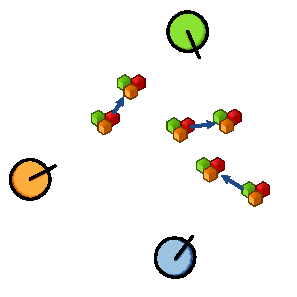
\includegraphics[scale=0.75]{Figures/Mamot}};
			\end{tikzpicture}
		}
		
		\column{0.2\textwidth}
		\centering
		
		\only<2->
		{
			\begin{tikzpicture}
				\node at (0,0) [draw=white,ultra thick,inner sep=0pt]  {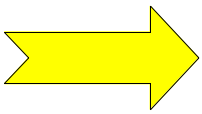
\includegraphics[scale=0.3]{Figures/ArrowRight.png}};
			\end{tikzpicture}
		}
		
		\column{0.4\textwidth}
		\centering
		
		\only<2>
		{
			\begin{tikzpicture}
				\node at (0,0) [draw=black,ultra thick,inner sep=0pt]  {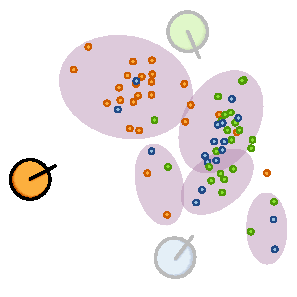
\includegraphics[scale=0.75]{Figures/Mamot2}};
			\end{tikzpicture}
		}
		
		\only<2>
		{
			\vspace{-0.7cm}
		}
		
		\only<3>
		{
			\begin{tikzpicture}
				\node at (0,0) [draw=black,ultra thick,inner sep=0pt]  {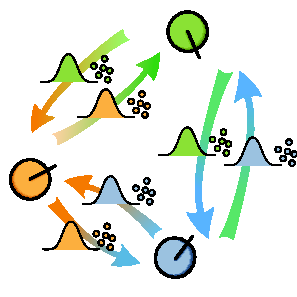
\includegraphics[scale=0.75]{Figures/Mamot3}};
			\end{tikzpicture}
		}
		
		\only<3>
		{
			\vspace{-0.7cm}
		}
		
		\only<4>
		{
			\begin{tikzpicture}
				\node at (0,0) [draw=black,ultra thick,inner sep=0pt]  {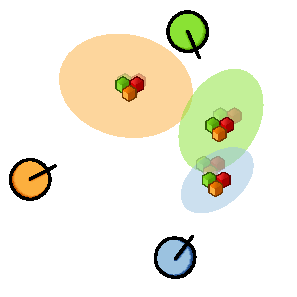
\includegraphics[scale=0.75]{Figures/Mamot4}};
			\end{tikzpicture}
		}
		
		\only<4>
		{
			\vspace{-0.7cm}
		}
	\end{columns}
\end{frame}

\begin{frame}
	\frametitle{Application fields}
	
	\vspace{0.24cm}
	
	\begin{itemize}
		\item Multi-Robot, Single-Object
	\end{itemize}
	
	\vspace{-0.45cm}
	
	\begin{columns}[t]
		\only<1->
		{
			\column{0.75\textwidth}
			
			\begin{block}{Soccer robots}
				used to solve the localization field symmetry problem
			\end{block}
			
			\column{0.2\textwidth}
		}
	\end{columns}
	
	\centering
	\vspace{0.3cm}
	
	\begin{tikzpicture}
				\node at (0,0) [draw=black,ultra thick,inner sep=0pt]  {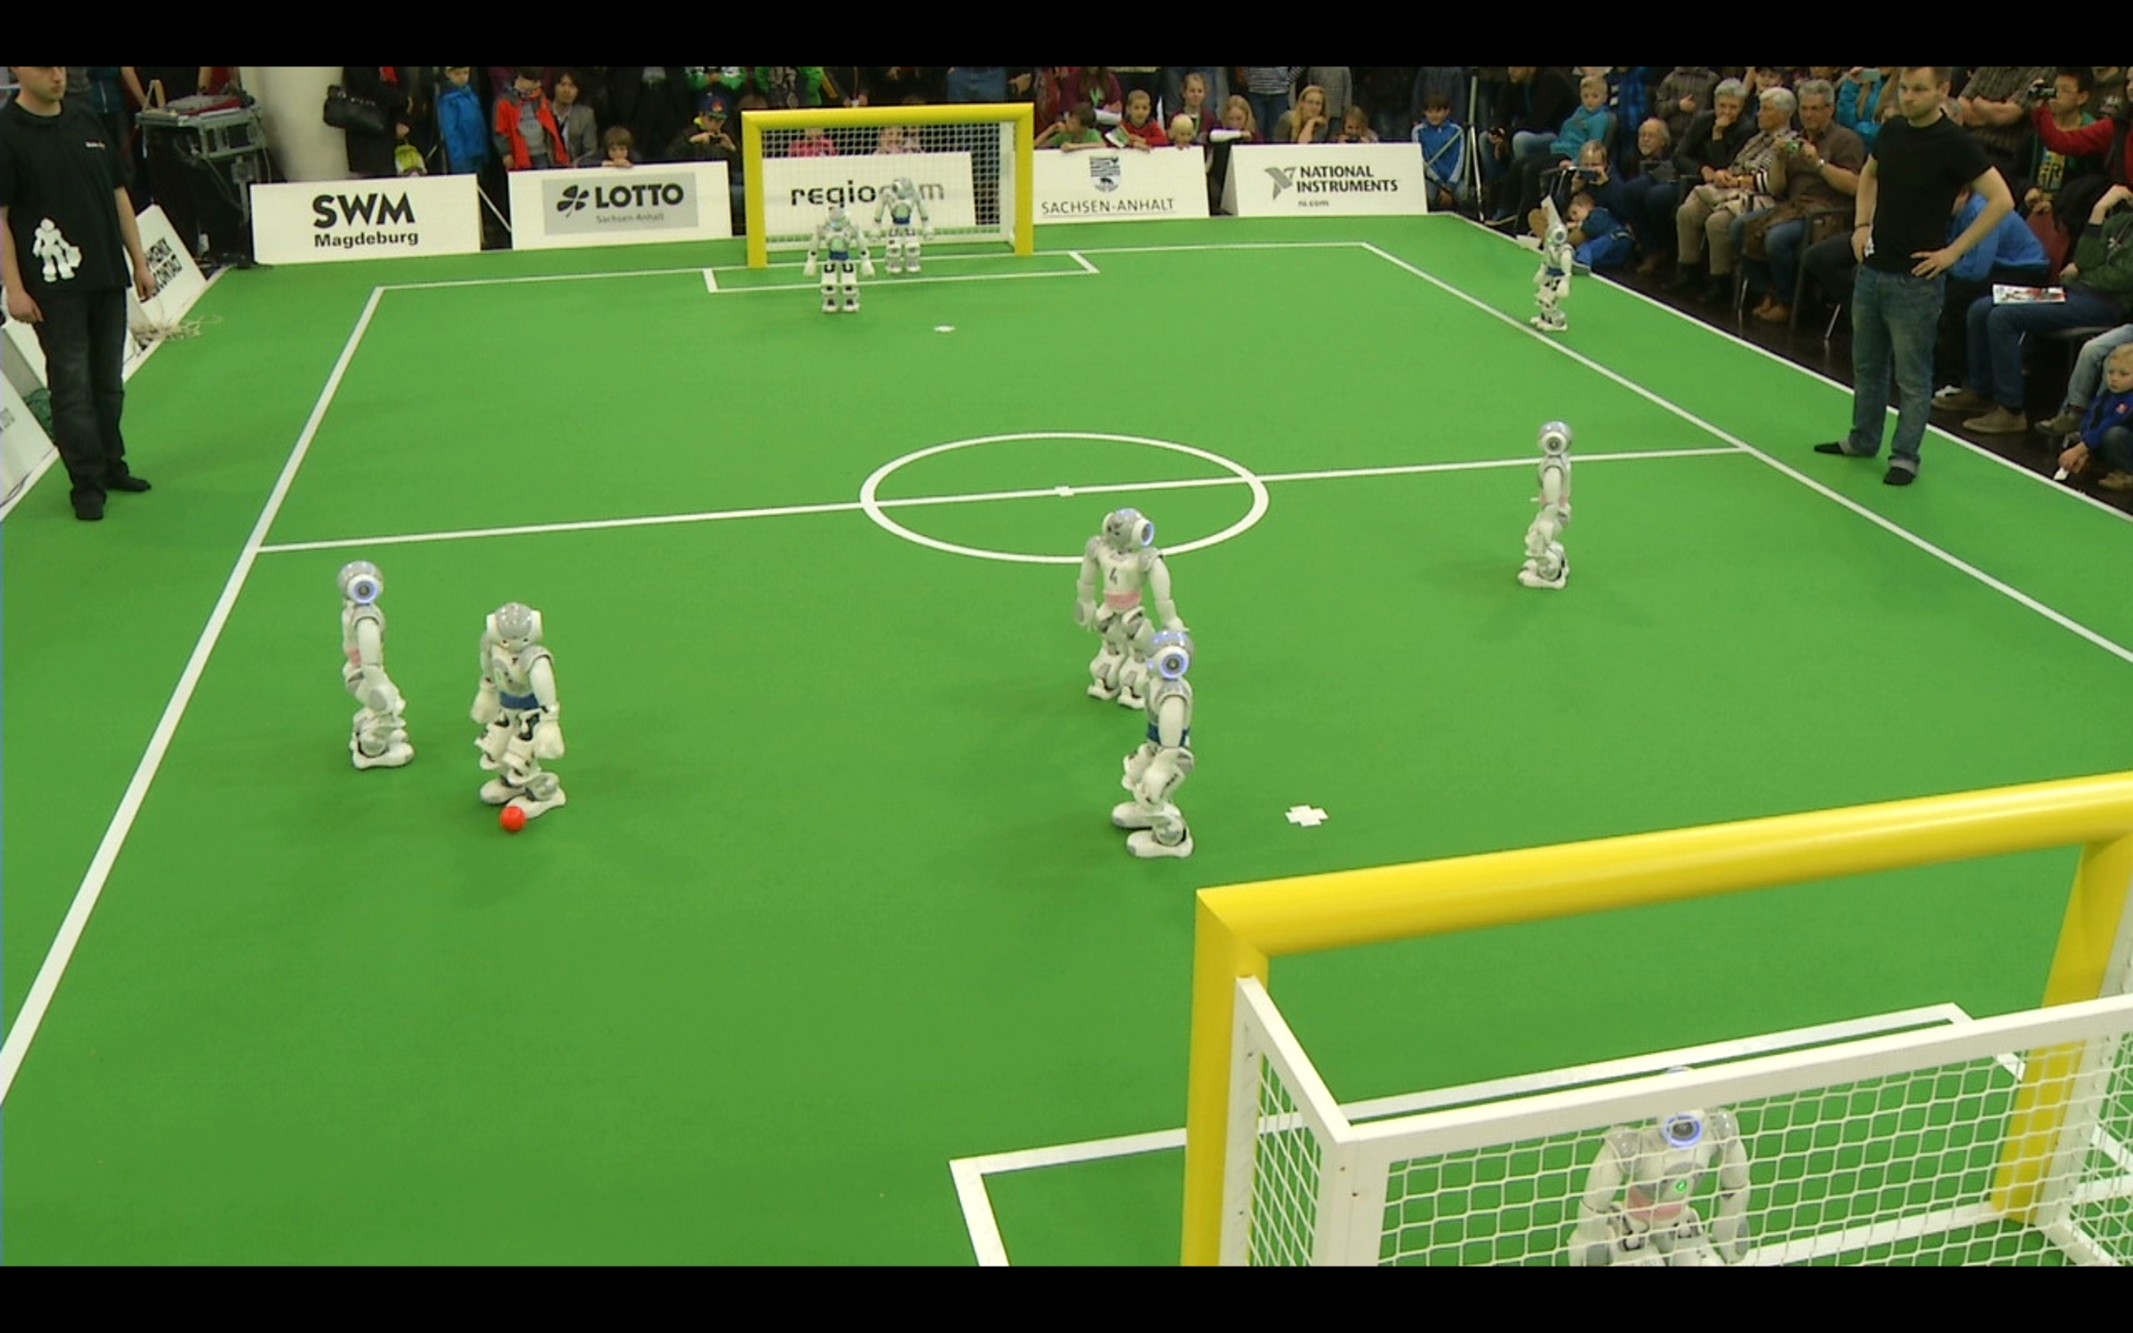
\includegraphics[scale=0.19]{Figures/Naos}};
	\end{tikzpicture}
	
\end{frame}

\begin{frame}
	\frametitle{Application fields}
	
	\vspace{0.455cm}
	
	\begin{itemize}
		\item Multi-Robot, Multi-Object
	\end{itemize}
	
	\vspace{-0.455cm}
	
	\begin{columns}[t]
		\only<1->
		{
			\column{0.35\textwidth}
			\centering
			
			\begin{block}{Prey-Predator game}
				Player/Stage
			\end{block}
			
			\column{0.6\textwidth}
			\centering
			
			\vspace{0.1cm}
			
			\begin{tikzpicture}[map/.style={draw=black,ultra thick,inner sep=0pt}]
				\node at (-3.9,0.8) [map] {
\includegraphics[height=1.1cm]{Maps/Edmonton}};
				\node at (-4.3,1.3) [map] {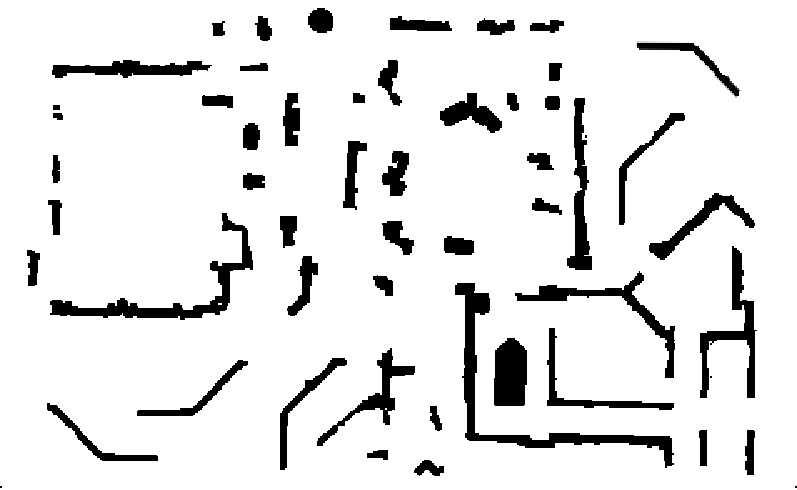
\includegraphics[height=1.1cm]{Maps/Longwood}};
				\node at (-3.0,1.0) [map] {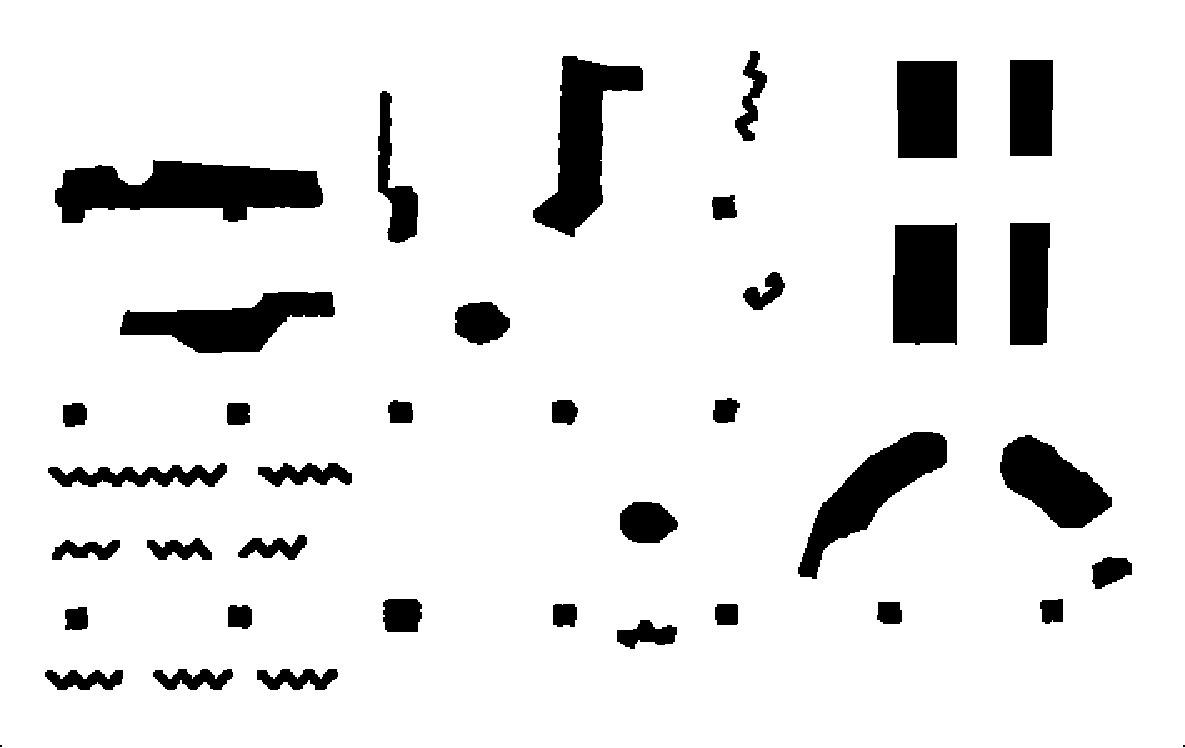
\includegraphics[height=1.1cm]{Maps/Mexico}};
				\node at (-2.8,1.5) [map,draw=red!70!black] {
\includegraphics[height=1.25cm]{Maps/Lasermaze}};
			\end{tikzpicture}
		}
	\end{columns}
	
	\vspace{-0.75cm}
	
	\begin{columns}[t]
		\only<1->
		{
			\column{0.55\textwidth}
			\centering
			
			\vspace{0.55cm}
			
			\begin{block}{PETS 2009 dataset}
				Tracking of individuals within a crowd
			\end{block}
			
			\column{0.4\textwidth}
		}
	\end{columns}
	
	\begin{center}
		\begin{tikzpicture}
			\node at (0,0) [draw=black,ultra thick,inner sep=0pt]  {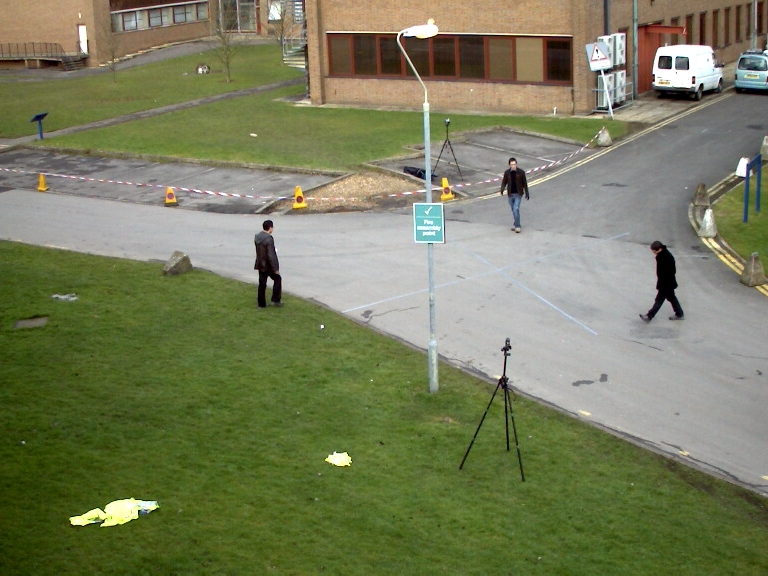
\includegraphics[scale=0.14]{Figures/Pets2009-1.jpg}};
			\node at (4,0) [draw=black,ultra thick,inner sep=0pt]  {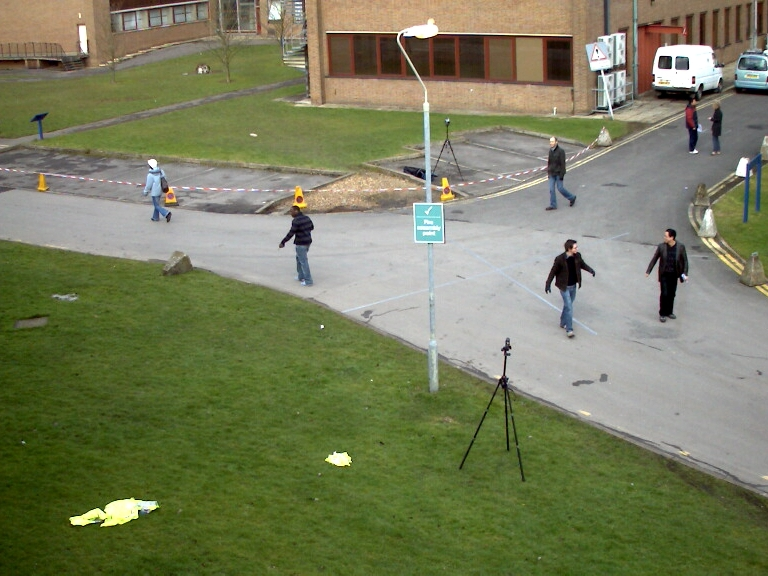
\includegraphics[scale=0.14]{Figures/Pets2009-2.jpg}};
			\node at (8,0) [draw=black,ultra thick,inner sep=0pt]  {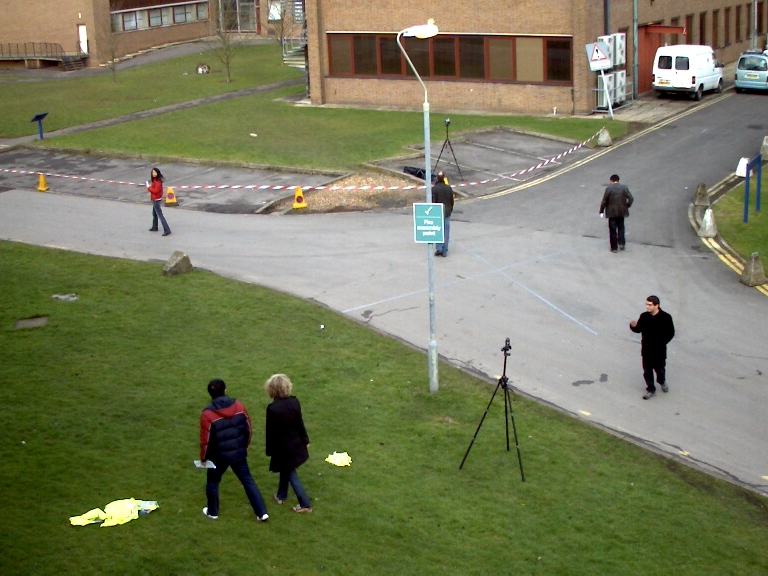
\includegraphics[scale=0.14]{Figures/Pets2009-3.jpg}};
		\end{tikzpicture}
	\end{center}
\end{frame}

\begin{frame}
	\frametitle{A learning approach to Multi-Object Detection and Tracking}
	
	\vspace{-2.5cm}
	
	\only<1->
	{
		\begin{block}{Goal}
			Creating a system that \textbf{can track} objects in an environment using sensors and that is \textbf{able to learn} the behaviours of the tracked objects by applying learning techniques
		\end{block}
	}
	
	\only<2->
	{
		\begin{itemize}
			\item \large\textcolor{red}{Unexplored} open field
		\end{itemize}
	}
	
	\only<2>
	{
		\vspace{-1cm}
	}
	
	\only<3>
	{
		\begin{itemize}
			\item \large\textcolor{red}{Challenges}
			
			\begin{itemize}
				\item \large\textcolor{red}{real-time} object motion detection
				\item objects' \large\textcolor{red}{behavior} recognition
			\end{itemize}
		\end{itemize}
	}
	
	\only<3>
	{
		\vspace{-3.07cm}
	}
\end{frame}

\begin{frame}
	\frametitle{Non-adaptive tracking}
	\framesubtitle{Current state of the art}
	
	\vspace{-3.0cm}
	
	\begin{columns}[t]
		\column{0.7\textwidth}
		
		\only<1->
		{
			\vspace{0.22cm}
		}
		
		\only<1->
		{
			\begin{itemize}
				\item Car park monitoring
				\vspace{0.1cm}
				\newline
				\tiny[\emph{Hampapur et al, ``Smart video surveillance: exploring the concept of multiscale spatiotemporal tracking'', 2005}]
			\end{itemize} 
		}
		
		\only<2->
		{
			\vspace{0.41cm}
		}
		
		\only<2->
		{
			\begin{itemize}
				\item Small objects tracking in aerial video sequences
				\vspace{-0.14cm}
				\newline
				\tiny[\emph{Pless et al, ``Detecting independent motion: the statistics of temporal continuity'', 2000}]
			\end{itemize}
			
			\vspace{0.13cm}
			
			\begin{itemize}
				\item Surveillance system specialized in people tracking
				\vspace{0.1cm}
				\newline
				\tiny[\emph{Haritaoglu et al, ``$ W_4 $: real-time surveillance of people and their activities'', 2000}]
			\end{itemize}
		}
		
		\only<2>
		{
			\vspace{-3.18cm}
		}
		
		\column{0.3\textwidth}
		
		\only<1->
		{
			\begin{tikzpicture}
				\node at (0,0) [draw=black,ultra thick,inner sep=0pt]  {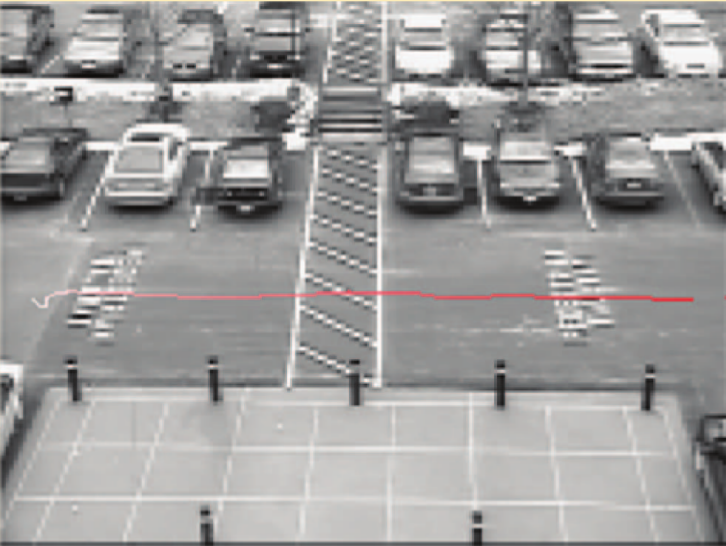
\includegraphics[width=2.3cm]{Figures/CarsPark.png}};
			\end{tikzpicture}
		}
		
		\only<2->
		{
			\begin{tikzpicture}
				\node at (0,0) [draw=black,ultra thick,inner sep=0pt]  {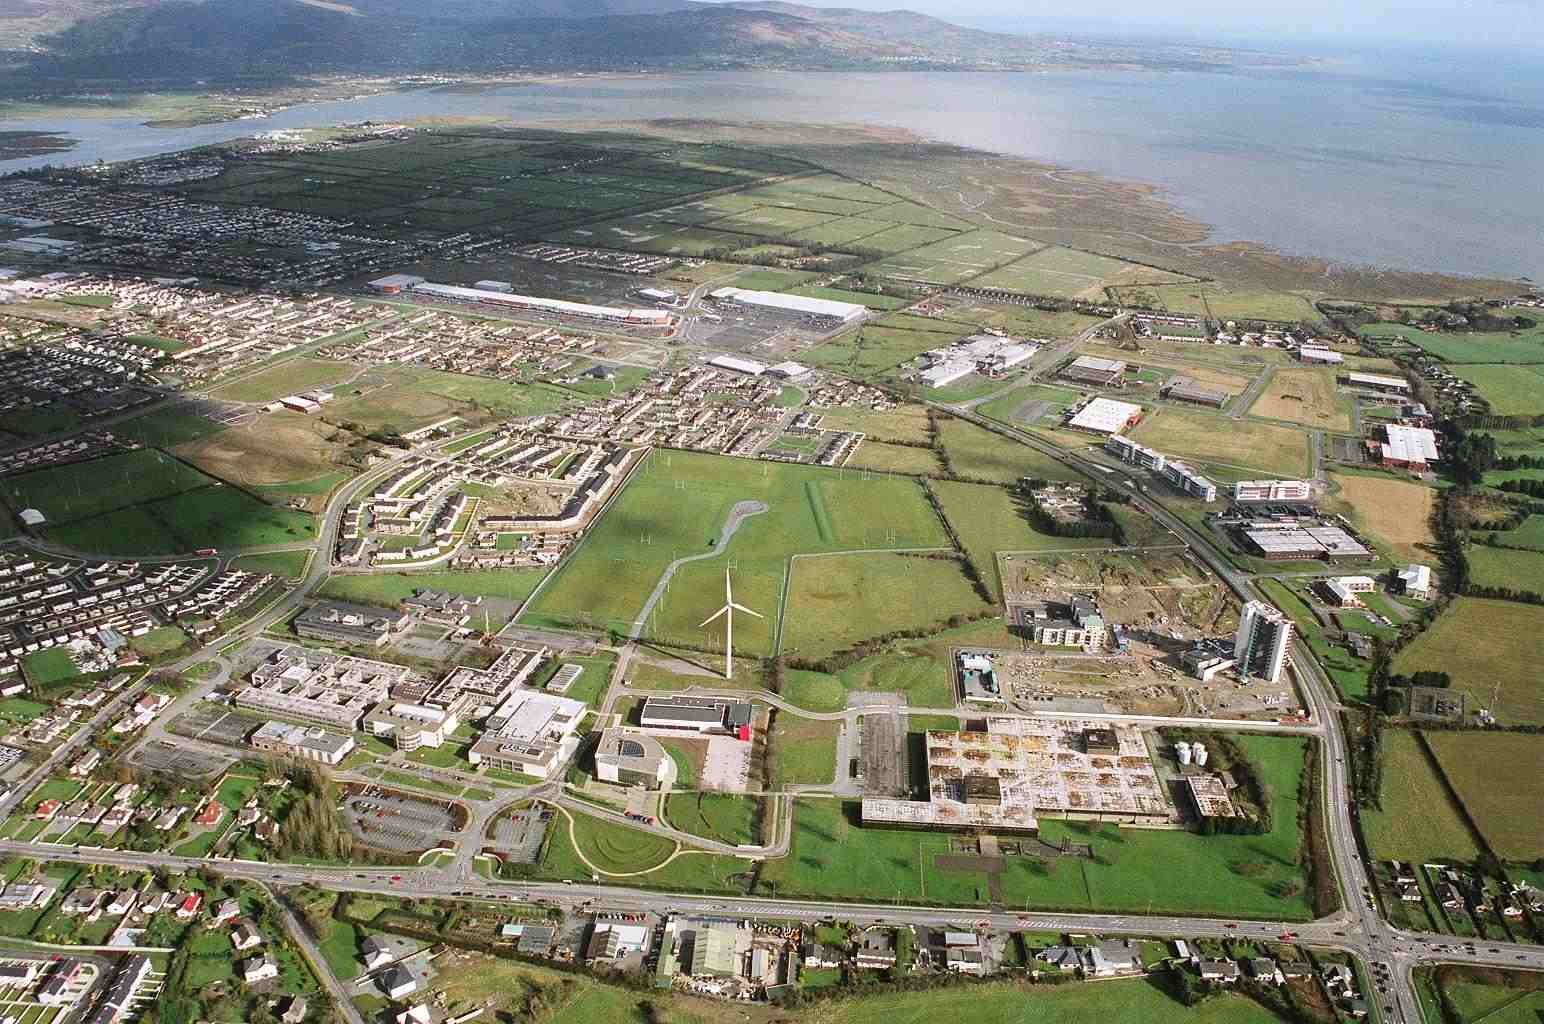
\includegraphics[width=2.3cm]{Figures/Aerial.jpg}};
			\end{tikzpicture}
			
			\begin{tikzpicture}
				\node at (0,0) [draw=black,ultra thick,inner sep=0pt]  {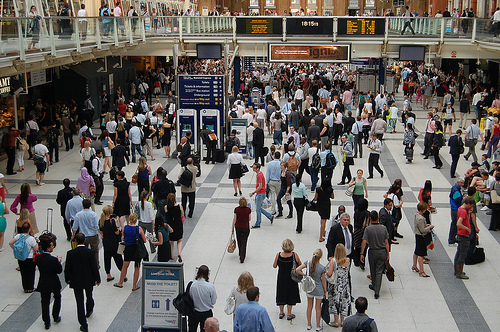
\includegraphics[width=2.3cm]{Figures/FollowingPeople.jpg}};
			\end{tikzpicture}
		}
		
		\only<2>
		{
			\vspace{-5.0cm}
		}
	\end{columns}
\end{frame}

\begin{frame}
	\frametitle{Adaptive tracking}
	
	\only<1>
	{
		\vspace{0.13cm}
	}
	
	\only<1->
	{
		\begin{itemize}
			\item Good results but \textbf{non-adaptive} tracking...
		\end{itemize}
		
		\vspace{-0.5cm}
		
		\begin{tabbing}
			\hspace*{1.0cm}
			
			$ \leadsto $ \textcolor{red}{weak} to environment's changes
		\end{tabbing}
	}
	
	\only<1>
	{
		\vspace{4.05cm}
	}
	
	\only<2->
	{
		\centering
		
		\vspace{-0.2cm}
		
		\begin{tikzpicture}
			\node at (0,0) [draw=white,ultra thick,inner sep=0pt]  {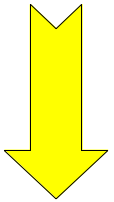
\includegraphics[scale=0.2]{Figures/ArrowDown.png}};
		\end{tikzpicture}
		
		\textcolor{red}{\textbf{Adaptive tracking}}
		
		\vspace{0.2cm}
		
		\begin{itemize}
			\item \textbf{Small} literature
		\end{itemize}
		
		\vspace{-0.5cm}
		
		\begin{tabbing}
			\hspace*{1.0cm}
			
			$ \leadsto $ \scriptsize[\emph{Stauffer et al, ``Learning patterns of activity using real-time tracking'', 2000}]
		\end{tabbing}
	}
\end{frame}

\begin{frame}
	\frametitle{A learning approach to Multi-Object Detection and Tracking}
	
	\only<1->
	{
		\vspace{-2.4cm}
	}
	
	\only<1->
	{
		An object tracking system \textbf{cannot} be used alone
		
		\begin{itemize}
			\item \emph{system setup}
			
			\item \emph{continuous maintenance after deployment}
		\end{itemize}
	}
	
	\only<2->
	{
		\centering
		
		\begin{tikzpicture}
			\node at (0,0) [draw=white,ultra thick,inner sep=0pt]  {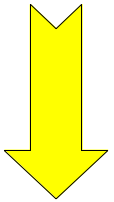
\includegraphics[scale=0.2]{Figures/ArrowDown.png}};
		\end{tikzpicture}
		
		\vspace{-0.4cm}
		
		\begin{center}
			\textcolor{red}{\textbf{adaptive smart tracking system}}
		\end{center}
		
		$ \leadsto $ the \textcolor{red}{better} is the experience, the \textcolor{red}{better} are the performance over time
	}
	
	\only<2>
	{
		\vspace{-2.99cm}
	}
\end{frame}

\section{Conclusions}

\begin{frame}
	\frametitle{Conclusions}
	
	\Large
	
	\vspace{0.3cm}
	
	We presented:
	
	\begin{enumerate}
		\item \emph{PTracking}, a novel \textbf{real-time} distributed tracker
		\item \textbf{Effective} framework for \textbf{predicting} future agent motions of
			  goal-oriented agents
	\end{enumerate}
	
	\vspace{0.2cm}
	
	\underline{\textbf{Main contributions}}
	
	\begin{itemize}
		\item Real-time, accurate and precise tracking
		\item Fully scalable design
		\item Prediction without prior annotation of scene semantics
		\item Non-uniform grids for state representation
		\item Efficient and scalable for on-robot implementation
	\end{itemize}
\end{frame}

\begin{frame}
	\frametitle{Future Work}
	
	\Large
	
	Possible future directions in terms of tracking could be:
	\begin{itemize}
		\item \textbf{Integration} of recent real-time \textbf{feature extractors} in the data
			  association module
		\item \textbf{Generation} of a \textbf{3D model} by merging information coming from multiple
			  sources
	\end{itemize}
	
	while, in terms of prediction of future agent motions could be the employment of \textbf{more
	sophisticated} \emph{IRL} alternatives within the overall proposed framework.\\
\end{frame}

\logo{}

\begin{frame}
	\frametitle{Major Reviewers' Comments}
	
	\large
	
	\textbf{Rev.}\\
	``For some experiments, comparisons are only made with various versions of the same algorithms.''
	
	\vspace{0.3cm}
	
	\textbf{Rev.}\\
	``The benefits of the method are shown for activity forecasting applications, intention prediction,
	and for constructing interactive costmaps to guide robot navigation. The latter applications
	represent significant contributions in robotics. Some additional discussion of the assumptions being  
	employed would be useful. Specifically, the joint optimization seems to assume more coordination
	than, e.g., humans have when they navigate (often sub-­optimally).'' \\
\end{frame}

\logo
{
	\begin{tikzpicture}
		\hspace{0.09cm}
		\node at (-1,0) [draw=white,ultra thick,inner sep=0pt]
		{
			
\includegraphics[height=1cm]{ThemeFigs/Sapienza}
		};
		\node at (0,0) [draw=white,ultra thick,inner sep=0pt]
		{
			
\includegraphics[height=1cm]{ThemeFigs/Edinburgh}
		};
	\end{tikzpicture}
	\vspace{199.1pt}
}

\begin{frame}
	\frametitle{Full List of Publications}
	
	\vspace{-0.2cm}
	
	\begin{columns}[t]
		\column{0.48\textwidth}
		
		\tiny
		
		\textcolor{red}{\textbf{\underline{Journal}}}
		
		\vspace{0.1cm}
		
		\textbf{1. Multi-Robot Surveillance through a Distributed Sensor Network}, A. Pennisi, F.
		Previtali, C. Gennari, D. D. Bloisi, L. Iocchi, F. Ficarola, A. Vitaletti, D. Nardi \\
		\emph{Journal of Studies in Computational Intelligence, 2015}
		
		\vspace{0.15cm}
		
		\textbf{2. Distributed Sensor Network for Multi-Robot Surveillance}, A. Pennisi, F. Previtali,
		F. Ficarola, D. D. Bloisi, L. Iocchi, A. Vitaletti \\
		\emph{Procedia Computer Science, 2014}
		
		\vspace{0.2cm}
		
		\textcolor{red}{\textbf{\underline{Conference}}}
		
		\vspace{0.1cm}
		
		\textbf{3. PTracking: Distributed Multi-Agent Multi-Object Tracking through Multi-Clustered
		Particle Filtering}, F. Previtali, L. Iocchi \\
		\emph{IEEE Conference on Multisensor Fusion and Integration, 2015}
		
		\vspace{0.15cm}
		
		\textbf{4. Disambiguating Localization Symmetry through a Multi-Clustered Particle Filtering},
		F. Previtali, G. Gemignani, L. Iocchi, D. Nardi \\
		\emph{IEEE Conference on Multisensor Fusion and Integration, 2015}
		
		\vspace{0.15cm}
		
		\textbf{5. Counterfactual Reasoning about Intent for Interactive Navigation in Dynamic
		Environments}, A. Bordallo, F. Previtali, N. Nardelli, S. Ramamoorthy \\
		\emph{IEEE Conference on Intelligent Robots and Systems, 2015}
		
		\vspace{0.15cm}
		
		\textbf{6. IRL-based Prediction of Goals for Dynamic Environments}, F. Previtali, A. Bordallo,
		S. Ramamoorthy \\
		\emph{Machine Learning for Social Robotics at ICRA, 2015}
		
		\column{0.53\textwidth}
		
		\vspace{0.34cm}
		
		\tiny
		
		\textbf{7. Real-Time Adaptive Background Modeling in Fast Changing Conditions}, A. Pennisi, F.
		Previtali, D. D. Bloisi, L. Iocchi \\
		\emph{Conference on Advanced Video and Signal based Surveillance, 2015}
		
		\vspace{0.2cm}
		
		\textcolor{red}{\textbf{\underline{Submitted}}}
		
		\vspace{0.1cm}
		
		\textbf{8. A Distributed Approach for Real-Time Multi-Camera Multi-Object Tracking}, F.
		Previtali, D. D. Bloisi, L. Iocchi \\
		\emph{Journal on Machine Vision and Applications}
		
		\vspace{0.15cm}
		
		\textbf{9. Enhancing Automatic Maritime Surveillance Systems with Visual Information}, D. D.
		Bloisi, F. Previtali, A. Pennisi, D. Nardi, M. Fiorini \\
		\emph{Transaction on Intelligent Transportation Systems}
		
		\vspace{0.15cm}
		
		\textbf{10. Predicting Future Agent Motions for Dynamic Environments}, F. Previtali, A.
		Bordallo, L. Iocchi, S. Ramamoorthy \\
		\emph{IEEE Conference on Intelligent Robots and Systems}
		
		\vspace{0.15cm}
		
		\textbf{11. Interactive Costmaps: Integrating Prediction and Planning with Counterfactual
		Reasoning}, A. Bordallo, F. Previtali, S. Ramamoorthy \\
		\emph{IEEE Conference on Intelligent Robots and Systems}
	\end{columns}
\end{frame}

\logo{}

\begin{frame}
	\frametitle{That's all!}
	
	\begin{figure}
		\centering
		\begin{tikzpicture}
			\node at (0,0) [draw=white,ultra thick,inner sep=0pt]
			{
				
\includegraphics[width=0.8\linewidth]{Figures/Question}
			};
		\end{tikzpicture}
	\end{figure}
\end{frame}


\tiny
\bibliographystyle{plain}
\bibliography{PTracking}
\nocite{Hampapur05}
\nocite{Pless00}
\nocite{Haritaoglu00}
\nocite{Stauffer00}

\end{document}
